\documentclass[10pt,twocolumn]{article}

\usepackage[T1]{fontenc}
\usepackage[margin=0.72in,columnsep=0.23in]{geometry}
\usepackage{amsmath,amssymb}
\usepackage{booktabs}
\usepackage{tabularx}
\usepackage{xcolor}
\usepackage{graphicx}
\usepackage[hidelinks]{hyperref}
\hypersetup{
  pdftitle={FinLeakAudit: Evidence-Level Point-in-Time Auditing for Financial Agentic RAG},
  pdfauthor={Ziyang Lu, Junwei Chen, Yating Zhang}
}

\newcolumntype{Y}{>{\raggedright\arraybackslash}X}

\newcommand{\system}{FinLeakAudit}
\newcommand{\up}{\textsc{up}}
\newcommand{\down}{\textsc{down}}
\newcommand{\neutral}{\textsc{neutral}}
\newcommand{\clean}{\textsc{Clean}}
\newcommand{\unfiltered}{\textsc{Unfiltered}}
\newcommand{\sparse}{\textsc{Sparse}}
\newcommand{\backfill}{\textsc{Backfilled}}

\title{FinLeakAudit: Evidence-Level Point-in-Time Auditing\\
for Financial Agentic RAG}
\author{
Ziyang Lu$^{1,*}$ \quad Junwei Chen$^{2}$ \quad Yating Zhang$^{3}$\\
\scriptsize $^{1}$The Hong Kong University of Science and Technology \quad
$^{2}$Johns Hopkins University \quad $^{3}$South China Normal University\\[-1pt]
\scriptsize $^{*}$Corresponding author: \texttt{zluca@connect.ust.hk}
}
\date{}

\begin{document}
\raggedbottom
\maketitle

\begin{abstract}
Financial forecasting systems built on retrieval-augmented large language models can
silently consume evidence that was unavailable at a historical prediction cutoff.
This can produce plausible rationales and inflated backtests without preserving the
information set available to a real decision maker. We present \system{}, an
evidence-level audit protocol separating point-in-time availability, citation
validity, claim--evidence attribution, marginal forecast sensitivity, and
leakage-driven revision. In a controlled 10-case study across three LLMs,
post-cutoff evidence was cited in 28/30 model-case runs and changed 12/30 forecast
categories; removing it restored the corresponding cutoff-safe category in 12/12
changed runs. A 10-event primary-source replay produced 13 changes in 30 model-event
runs. Sparse deletion recovered 11/13, while rank-preserving cutoff-safe backfill
recovered 13/13 and matched the Clean direction in 30/30 runs. However, 24/30
backfilled inputs were identical to Clean and the exact paired McNemar test was not
significant ($p=0.25$). On 78 decisive human-labeled claim--evidence pairs,
citation-only attribution achieved F1 0.941 and a blinded LLM judge achieved F1
0.937. The results provide a reproducible audit pilot and expose concrete failure
modes; they do not estimate real-world leakage prevalence or demonstrate improved
forecasting accuracy.
\end{abstract}

\section{Introduction}

Retrieval-augmented generation (RAG) gives language models access to explicit
non-parametric evidence and provenance \cite{lewis2020rag}. In financial forecasting,
that evidence must also obey a historical information boundary: a document is usable
only if it was available by the prediction cutoff. Agentic RAG complicates this
requirement because retrieval, synthesis, citation, and forecast revision can each
introduce or conceal look-ahead information.

Recent systems combine LLM agents with filings, earnings calls, news, and structured
financial context \cite{fatouros2025marketsenseai,li2026carag}. At the same time,
financial-LLM studies report memorization-driven profit inflation and decision-time
availability failures \cite{li2025profitmirage,benhenda2026lookahead,guan2026leakageaware}.
These works motivate a narrower question: when a retrieved item postdates the cutoff,
can we trace whether the forecast used it, measure its marginal impact, and revise the
forecast without silently changing the evaluation target?

\system{} is designed as an audit layer for host Agentic RAG systems. The present
pilot evaluates their retrieval-grounded forecasting interface under fixed retrieval;
it does not exercise autonomous query reformulation, tool planning, or multi-agent
coordination.

We study four research questions:
\begin{enumerate}
  \item Does post-cutoff evidence alter forecasts under controlled injection?
  \item Does the effect appear in a small replay built from archived primary sources?
  \item Does deletion restore the cutoff-safe prediction, and can deletion itself
        introduce revision instability?
  \item How well do citation, lexical, embedding, and LLM-based methods identify
        claim--evidence dependence?
\end{enumerate}

Our contributions are deliberately bounded. First, we define an evidence-level
point-in-time audit protocol with separate predictor, auditor, and evaluator views.
Second, we introduce paired \clean{}, contaminated, \sparse{}, and \backfill{}
conditions that distinguish leakage recovery from deletion-induced drift. Third, we
release a reproducible pilot spanning three models, two forecast stress tests, a
human-labeled attribution set, and failure-preserving logs.

\section{Related Work}

\paragraph{Financial forecasting with LLMs.}
SEP trains self-reflective LLMs to produce explainable stock predictions
\cite{koa2024sep}. MarketSenseAI 2.0 combines agents and RAG over news, prices,
fundamentals, filings, and macroeconomic material \cite{fatouros2025marketsenseai}.
CARAG retrieves structured evidence from a causal-temporal knowledge graph for
post-earnings price-shock prediction \cite{li2026carag}, while TRACE produces
temporally grounded knowledge-graph evidence chains \cite{ding2026trace}. These are
forecasting systems; \system{} instead audits the evidence boundary of a host
forecasting workflow.

\paragraph{Temporal leakage in financial AI.}
Profit Mirage diagnoses memorization-driven leakage through counterfactual tests and
out-of-window generalization \cite{li2025profitmirage}. Look-Ahead-Bench compares
in-sample and out-of-sample agent performance using alpha decay
\cite{benhenda2026lookahead}. Their reported unit of diagnosis is model or agent
behavior across periods. \system{} instead holds the predictor fixed and intervenes
on its retrieved context: it verifies when each item became available, links that
item to generated claims, and tests whether removal changes or restores the forecast.
The approaches are therefore complementary rather than competing forecasting
benchmarks. Leakage-aware macro factor ranking distinguishes target timestamps from
decision-time observability \cite{guan2026leakageaware}, while OpenFinGym prevents
runtime train--test leakage at the execution boundary \cite{zhang2026openfingym}.

\paragraph{Attribution, verification, and revision.}
ALCE evaluates whether generated claims carry correct and complete citations
\cite{gao2023alce}. Evidence ablation in LLM forecasters shows that a forecast can
change while its stated reasoning remains stable \cite{sarfati2026forecasters}, which
motivates separating explicit citation from behavioral sensitivity. In finance,
VERAFI validates calculations and regulatory constraints \cite{akinfaderin2025verafi},
and SHARP audits and edits human-readable trading rules \cite{chen2026sharp}.
FLAIRR-TS revises forecasting prompts to improve accuracy
\cite{jalori2025flairr}. Our revision trigger is neither policy performance nor
prediction error; it is evidence unavailability at the historical cutoff.

\section{Problem Formulation}

For event $j$, let $\tau_j$ denote the prediction cutoff, $h_j$ the forecast
horizon, and $E_j=\{e_1,\ldots,e_k\}$ the retrieved evidence. Each item has a
verifiable availability time $a(e_i)$. Its point-in-time validity is
\begin{equation}
  v(e_i;\tau_j)=\mathbb{1}[a(e_i)\leq\tau_j].
\end{equation}
A predictor $f$ maps predictor-visible evidence text and IDs to a categorical
forecast $y\in\{\up,\down,\neutral\}$, confidence, claims, and cited IDs. The
predictor never sees availability timestamps, audit labels, or outcomes.

We compare four conditions. \clean{} retrieves cutoff-safe top-$k$ evidence.
\unfiltered{} retrieves up to the outcome boundary and may contain future items.
\sparse{} removes all known post-cutoff items from the actual \unfiltered{} set.
\backfill{} preserves the surviving order and fills empty slots with the highest
ranked cutoff-safe items not already present.

An initial flip occurs when $y_C\neq y_U$. Recovery is defined only on flips and
requires $y_R=y_C$. Revision drift is defined only when $y_C=y_U$ but $y_R\neq y_C$.
Leave-one-out reruns are reported as marginal sensitivity, not causal effects.

\section{Audit Protocol}

\begin{figure*}[t]
\centering
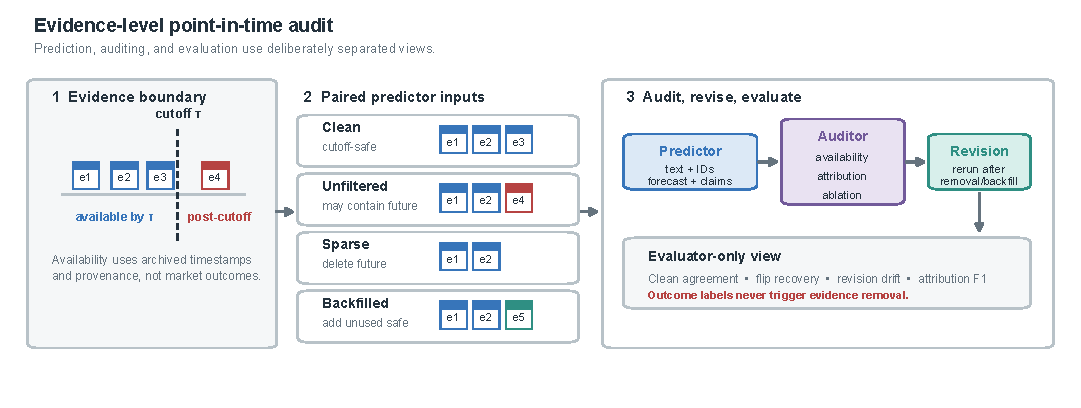
\includegraphics[width=0.98\textwidth]{figures/finleakaudit_pipeline.pdf}
\caption{The FinLeakAudit protocol. A historical cutoff separates available from
post-cutoff evidence. Paired predictor inputs isolate contamination and revision,
while the auditor and evaluator receive distinct views. Outcome labels never enter
prediction, evidence removal, or Backfill selection.}
\label{fig:pipeline}
\end{figure*}

\paragraph{Availability and visibility.}
The temporal operator receives timezone-aware timestamps and provenance. The
predictor receives only evidence IDs and text. The evaluator alone receives outcome
labels. Natural cases use archived primary-source timestamps with independent human
cross-checking. Market-calendar alignment and revision/vendor timestamp modeling are
not yet complete.

\paragraph{Citation and semantic attribution.}
Cited strings are checked against exact IDs shown to the predictor. Shortened,
fabricated, or concatenated IDs are retained as failures rather than normalized.
For each claim and post-cutoff candidate, semantic attribution compares the claim,
candidate text, and pre-cutoff evidence without revealing model, event, timestamp,
citation, or outcome metadata. Candidate support is distinguished from dependence
exclusive to the post-cutoff item.

\paragraph{Revision.}
Known-unavailable items are removed by the temporal operator. \sparse{} revision
tests direct deletion. \backfill{} tests whether observed changes are partly due to
reduced context size rather than removal itself. Backfill never uses the outcome or
manual sentiment labels.

\section{Data and Experimental Setup}

\begin{table}[t]
\centering
\small
\begin{tabularx}{\columnwidth}{@{}lrrY@{}}
\toprule
Set & Items & Runs & Purpose \\
\midrule
Controlled injection & 10 cases & 30 & Premise and pipeline check \\
Natural replay & 10 events & 30 & Archived-source stress test \\
Attribution gold & 79 pairs & 79 & Claim--evidence evaluation \\
\bottomrule
\end{tabularx}
\caption{Evaluation assets. A run is one case/event evaluated by one model.}
\label{tab:data}
\end{table}

The controlled set includes seven cases whose pre- and post-cutoff text is paraphrased
from verified SEC filings, and three semi-real cases with synthetic pre-cutoff context
and a verified company or regulatory event source. Each case contains one designed
post-cutoff item and serves as a stress test rather than a prevalence sample.

\paragraph{Natural candidate-feed corpus.}
The natural replay contains 189 candidate documents across ten real financial events,
covering earnings and guidance, cybersecurity, management changes, acquisitions, and
litigation. Version-aware extraction produced 201 retrieval units: 195 active units
and six webpage units excluded because their historical content could not be verified
reliably. A dynamic status page can produce several independently timestamped units,
so unit and document counts need not match. Event queries and cutoffs were frozen
before retrieval. Here, \emph{natural} denotes real events and source documents, not a
preserved search-engine result page or host Agentic-RAG trace.

\begin{table}[t]
\centering
\scriptsize
\begin{tabularx}{\columnwidth}{@{}llYcr@{}}
\toprule
Event & Type & Cutoff basis & $h$ & D/U \\
\midrule
CrowdStrike & Cyber & Previous close & $+1$ & 18/24 \\
NVIDIA & Earnings & Pre-release & $+1$ & 20/20 \\
NIKE & Earnings & Pre-release & $+1$ & 19/19 \\
Starbucks & Leadership & Pre-disclosure & $+3$ & 19/19 \\
Intel & Leadership & Pre-disclosure & $+2$ & 19/19 \\
Exxon Mobil & M\&A & Pre-disclosure & $+1$ & 19/19 \\
Capital One & M\&A & Pre-disclosure & $+1$ & 20/20 \\
Microsoft & M\&A & Pre-disclosure & $+1$ & 18/18 \\
UnitedHealth & Cyber & Pre-disclosure & $+3$ & 18/18 \\
JetBlue & Litigation & Pre-decision & $+2$ & 19/19 \\
\bottomrule
\end{tabularx}
\caption{Natural candidate-feed corpus. Horizon $h$ is measured in trading-day
closes; D/U gives candidate documents / active retrieval units.}
\label{tab:natural-corpus}
\end{table}

\paragraph{Retrieval implementation.}
HTML, XML, and PDF sources are deterministically extracted and split into chunks of at
most 4,000 characters with 300-character overlap. At most three time-ordered units per
parent source enter ranking. Frozen query terms are scored with log-scaled term
frequency and inverse document frequency; chunk IDs break ties deterministically.
The top-eight context admits at most two chunks per parent source. \clean{} retrieval
is bounded by the prediction cutoff, whereas \unfiltered{} retrieval is bounded by the
outcome time.

We evaluate DeepSeek \texttt{deepseek-chat}, Zhipu
\texttt{glm-4-flashx-250414}, and Qwen2.5-14B-Instruct GGUF Q4\_K\_M through
llama.cpp, all at temperature zero. Natural runs were executed between August 19 and
September 6, 2026; one Qwen timeout required a recorded second attempt. API aliases do
not expose immutable serving checkpoints, and provider-side determinism is not
assumed. Prompts, retrieval policies, model outputs, retries, token usage, and
malformed citations are retained.

\paragraph{Human verification and annotation.}
One researcher prepared the source, timestamp, and retrieval-unit metadata. A second
researcher independently reviewed 139 records selected by a frozen rule: every
post-cutoff or unresolved record and a deterministic sample of at least 20\% of each
event's pre-cutoff records. The review accepted 133 records, rejected one timestamp,
and sent five to coordinator adjudication; all six non-accept outcomes were resolved
before the replay was frozen. This is independent verification of the defined sample,
not dual review of every candidate document.

The attribution set contains 79 claim--post-cutoff-evidence pairs constructed from
controlled-run model claims. Two humans labeled the blind batch without model, event,
timestamp, citation, prediction-outcome, or automatic-audit metadata. The adjudicated
gold set contains 41 positive, 37 negative, and one uncertain pair; the uncertain pair
is excluded from binary evaluation. DeepSeek \texttt{deepseek-chat} is the blinded LLM
judge and receives only the claim, pre-cutoff evidence, and candidate post-cutoff
evidence.

\section{Results}

\begin{figure*}[t]
\centering
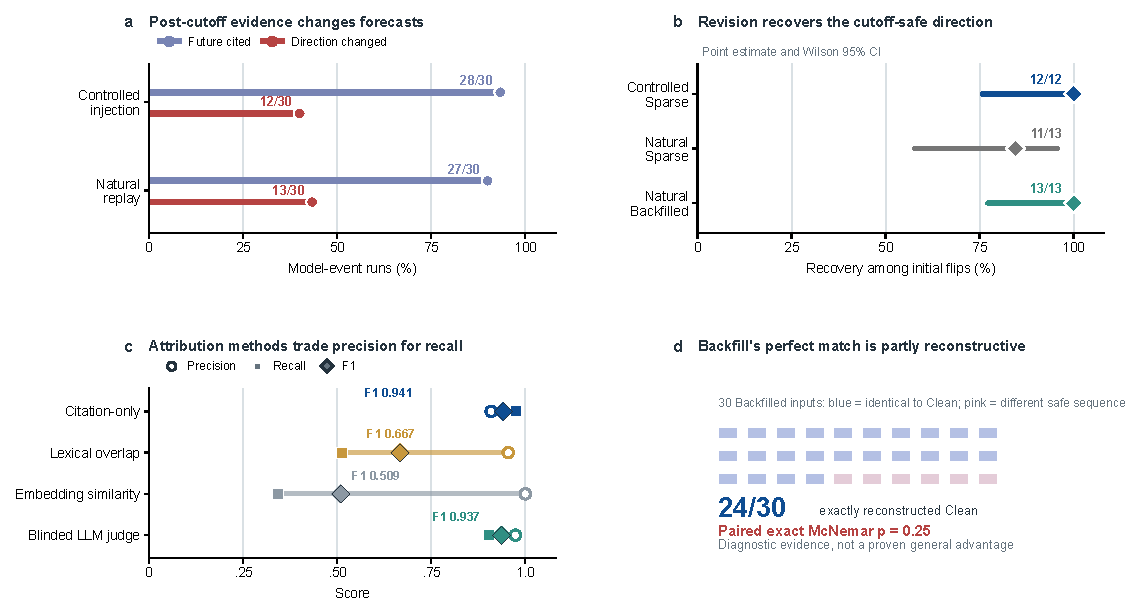
\includegraphics[width=0.98\textwidth]{figures/finleakaudit_results.pdf}
\caption{Audit and attribution results. \textbf{a}, Post-cutoff evidence citation
and forecast-direction changes over 30 runs per study. \textbf{b}, Conditional
recovery after revision; points show proportions and lines show Wilson 95\%
intervals. \textbf{c}, Precision, recall, and F1 on 78 decisive claim--evidence
pairs. \textbf{d}, Backfill interpretation: 24/30 Backfilled inputs exactly
reconstructed Clean, and the paired exact McNemar test was not significant. Exact
counts remain primary; Wilson intervals are descriptive because three models share
each event and evidence pool.}
\label{fig:results}
\end{figure*}

\subsection{Controlled Evidence Injection}

Across 30 model-case runs and 210 calls, models cited the future item in 28/30 runs
and changed category in 12/30. Removing temporally invalid evidence restored the
Clean category in 12/12 changed runs (Wilson 95\% interval 75.7\%--100\%). Clean,
contaminated, and audited outcome accuracy was 8/30, 18/30, and 8/30. The temporary
increase is induced hindsight inflation, not valid forecasting performance.

\subsection{Natural Point-in-Time Replay}

Across 30 model-event runs and 120 retained predictions, future evidence was
explicitly cited in 27/30 Unfiltered runs and changed direction in 13/30. Sparse
deletion recovered 11/13. Backfill recovered 13/13 (Wilson 95\% interval
77.2\%--100\%) and matched Clean in 30/30 runs (88.6\%--100\%). On 17 non-flipped
runs, Sparse drifted once and Backfill never drifted.

The 30 model-event observations are not independent because three models share each
event, retrieval query, and evidence pool. We therefore treat exact counts as primary
and Wilson intervals as descriptive summaries rather than event-independent
inferential estimates.

Backfill corrected three observed Sparse mismatches: DeepSeek on Intel, Qwen on
Exxon, and Qwen on Capital One. However, Backfilled evidence sequences exactly
matched Clean in 24/30 runs. The paired exact McNemar test gives $p=0.25$, so the
sample does not establish a general Backfill advantage. Outcome accuracy was 11/30
Clean, 16/30 Unfiltered, 11/30 Sparse, and 11/30 Backfilled.

Citation validation found 30 invalid IDs across 11/90 base-condition outputs and
eight invalid IDs across 3/30 Backfilled outputs. One Qwen event-level timeout was
retained and successfully retried. These failures are part of the measured interface,
not post-processing noise.

\subsection{Claim--Evidence Attribution}

Citation-only, lexical-overlap, embedding-similarity, and blinded-LLM attribution
achieved F1 scores of 0.941, 0.667, 0.509, and 0.937, respectively.
Citation-only attribution slightly exceeded the LLM judge on this controlled sample.
Its confusion counts were TP=40, FP=4, FN=1, and TN=33; the LLM judge produced TP=37,
FP=1, FN=4, and TN=36.
The aggregate masks complementary failures: exact matching missed a semantically used
future source whose chunk suffix was omitted, while the LLM judge produced a
support-without-dependence false positive when the same fact was already available
before cutoff. Annotator agreement on the original three-way semantic-dependence
label was 77/79, with Cohen's $\kappa=0.952$.

\begin{table*}[t]
\centering
\small
\begin{tabularx}{\textwidth}{@{}p{0.15\textwidth}p{0.27\textwidth}p{0.27\textwidth}Y@{}}
\toprule
Failure mode & Observed example & What a simple audit misses & Design consequence \\
\midrule
Malformed citation & Qwen described CrowdStrike's post-cutoff Falcon incident but
omitted required chunk suffixes. & Exact-ID matching recorded no valid future
citation although the rationale used the incident. & Evaluate citation validity and
semantic dependence as separate operators. \\
Redundant future support & A Zhipu Enphase claim cited post-cutoff shipment reductions,
but the inventory-glut premise was already explicit before cutoff. & A blinded LLM
judge labeled support as dependence, producing a false positive. & Compare each claim
against both pre- and post-cutoff evidence; support is not exclusive dependence. \\
Deletion-induced drift & Sparse deletion mismatched Clean for DeepSeek--Intel and
Qwen--Exxon, and created a Qwen--Capital One non-flip drift. & Removing invalid items
also changes context length and rank coverage. & Treat Backfill as a diagnostic
control, not a proven improvement. \\
\bottomrule
\end{tabularx}
\caption{Representative failure modes retained in the evaluation logs. The examples
motivate separate availability, attribution, and revision-stability measurements.}
\label{tab:failures}
\end{table*}

\section{Discussion}

The results support auditability, not forecasting superiority. Post-cutoff evidence
frequently changed predictions in both stress tests, and revision usually returned to
the cutoff-safe category. Yet timestamp filtering is intentionally strong when
availability is known exactly. Richer attribution matters when citations are
malformed, claims paraphrase sources, timestamps are uncertain, or the same claim is
supported on both sides of the cutoff.

The Sparse/Backfill comparison exposes a measurement confound: deletion can alter
context length, coverage, and rank distribution. Backfill removes three observed
Sparse mismatches, but it often reconstructs the Clean input and does not achieve a
significant paired advantage. It is therefore a diagnostic baseline, not a proven
improvement.

In an institutional deployment, the protocol can operate at two boundaries: a
pre-prediction gate that excludes evidence unavailable at the decision timestamp, and
a post-generation audit that validates citations, traces semantic dependence, and
triggers a controlled rerun. This complements model-level safety mechanisms without
requiring changes to the host predictor.

\section{Limitations and Ethics}

Ten events and 30 model-event observations are too small for prevalence claims. Event
selection is purposive and outcome-bounded. Controlled injections are easier than
production retrieval, and the natural replay is not a preserved web search or host
Agentic-RAG trace. The study does not evaluate autonomous planning, query rewriting,
tool selection, or multi-agent coordination. The semantic gold set is controlled; a
separately frozen natural hard set remains unlabeled and is not used in paper claims.
API aliases may change behind provider names, and temperature zero does not ensure
deterministic serving. Availability does not imply truthfulness or relevance. Market
outcomes are noisy and never determine evidence removal.

This work is a reliability benchmark rather than investment advice or a trading
system. Reproducibility records preserve provenance and hashes. Source documents are
redistributed only where source-specific terms permit; otherwise the release retains
canonical URLs, timestamps, and license notes.

\section{Conclusion}

\system{} operationalizes evidence-level point-in-time auditing for financial
Agentic RAG. Its paired conditions reveal both leakage-driven forecast changes and
revision-induced instability, while the attribution benchmark separates exact
citation from semantic dependence. The current study is a controlled pilot. Larger
natural event sets, frozen natural attribution labels, and host-system evaluations are
needed before broader claims.

\paragraph{Reproducibility.}
The project repository includes frozen cases, retrieval manifests, prompts, raw
outputs, error rows, analysis scripts, and tests. The AI4F submission snapshot is
available in a \href{https://github.com/yixi1120/FinLeakAudit-KB/tree/ai4f-2026-submission-v2}{versioned public repository}; artifact checksums and reproduction commands are
provided in its documentation. Source documents are redistributed only where their
terms permit; otherwise the snapshot records canonical URLs, timestamps, hashes, and
license notes.

\paragraph{Author contributions.}
Ziyang Lu led conceptualization, methodology, software, experiments, formal analysis,
visualization, annotation adjudication, writing, and project administration. Junwei
Chen curated the natural point-in-time corpus, prepared source and timestamp metadata
and retrieval units, and completed independent semantic annotation. Yating Zhang
completed independent semantic annotation and claim-span refinement, and independently
verified the frozen 139-record sample of natural-source metadata and timestamps.

\bibliographystyle{plain}
\bibliography{references}

\end{document}
